\documentclass[11pt]{article}
%\documentclass[11pt,twoside]{article}
\usepackage[letterpaper,margin=0.75in,left=1.25in,nohead]{geometry}
\usepackage{graphicx}
\usepackage{color}
\usepackage{amsmath}
\usepackage{amsfonts}
\usepackage{bbm}
\usepackage{tikz}
\usetikzlibrary{intersections}
\usepackage{subcaption}
\usepackage{mathrsfs}
\usepackage{mdframed}
\usepackage{makecell}

\usetikzlibrary{calc}
\def\centerarc[#1](#2)(#3:#4:#5)% Syntax: [draw options] (center) (initial angle:final angle:radius)
    { \draw[#1] ($(#2)+({#5*cos(#3)},{#5*sin(#3)})$) arc (#3:#4:#5); }

\begin{document}
\title{Complex Analysis: Exam 1B}
\author{Kevin Roebuck}
\maketitle

\begin{enumerate}
\item (20) Miscellaneous computations. Show all necessary steps.
  \begin{enumerate}
  \item Compute all values of $(1 - i)^{\frac{4}{3}} = ((1 - i)^4)^{\frac{1}{3}}$.

  \begin{mdframed}[align=left]
    Begin by writing $z = 1 - i$ in polar form. The modulus is $|z| = \sqrt{1^2 + (-1)^2} = \sqrt{2}$. Then, by using the relationships
    \begin{align*}
      \cos\theta = \frac{\text{Re}(z)}{|z|} \qquad \text{and} \qquad \sin\theta = \frac{\text{Im}(z)}{|z|},
    \end{align*}
    we see that $\cos\theta = 1/\sqrt{2}$ and $\sin\theta = -1/\sqrt{2}$. From this set of equations we conclude that Arg$(z) = -\pi/4$. Therefore $z = \sqrt{2}e^{-i\pi/4}$. Raising $z$ to the fourth power gives $z^4 = 4e^{-i\pi}$ = -4. Now all that's left to do is find the cube roots of $z^4$, which will require the use of
    \begin{equation*}
      z^{1/m} = |z|^{1/m}e^{i(\theta + 2k\pi)/m} \qquad (k = 0,1,2,...,m-1).
    \end{equation*}
    In our case $m = 3$ so that the above equation takes the form
    \begin{equation*}
      (z^4)^{1/3} = \left|z^4\right|^{1/3}e^{i(-\pi + 2k\pi)/3}
      = 4^{1/3}e^{i\pi(2k - 1)/3}
      \qquad (k = 0,1,2).
    \end{equation*}
    By plugging in the possible values of $k$, we get:

    \begin{center}
    \begin{tabular}{|l|l|}\hline
      $k$ & $z^{4/3}$ \\\Xhline{2\arrayrulewidth}
      0 & $4^{1/3}e^{-i\pi/3}$ \\\hline
      2 & $4^{1/3}e^{i\pi/3}$ \\\hline
      2 & $4^{1/3}e^{i\pi}$ \\\hline
    \end{tabular}
    \end{center}

    A plot of these roots, along with the vector representing $z^4$, can be seen in the figure below.

    \begin{center}
    \begin{tikzpicture} [scale=1.2]
      \draw[-] (0,0) -- (4,0); %draw axes
      \draw[-] (0,0) -- (0,4);
      \draw[line width=0.5mm, ->] (0,0) -- (-4,0); %draw z^4 vector
      %\draw[opacity=0.2] (0,0) circle(1.587cm); % draw circle
      \draw[line width=0.5mm, ->] (0,0) -- (-1.587,0); %draw cube root vectors
      \draw[line width=0.5mm, ->] (0,0) -- (0.793,-1.375);
      \draw[line width=0.5mm, ->] (0,0) -- (0.793,1.375);

      %draw labels
      \node at (4.2,0) {$x$};
      \node at (0,4.2) {$y$};
      \node at (-4.1,0.2) {$z^4$};
      \node at (1.7,-1.5) {$z^{4/3} (k=0)$};
      \node at (1.7,1.5) {$z^{4/3} (k=1)$};
      \node at (-1,0.3) {$z^{4/3} (k=2)$};
    \end{tikzpicture}
    \end{center}
  \end{mdframed}
  
  \item Compute ${\displaystyle \int_0^{2\pi}} \cos^5(x)\,dx$ using methods introduced in our class.
  
  \begin{mdframed}
    Start by simplifying the integrand using Euler's formula
    \begin{equation*}
      \cos^5 x = \left[\frac{e^{ix} + e^{-ix}}{2}\right]^5 = \frac{1}{2^5}[e^{ix} + e^{-ix}]^5.
    \end{equation*}
    Expanding via the binomial formula gives
    \begin{align*}
      \cos^5 x &= \frac{1}{2^5}[e^{5ix} + 5e^{4ix}e^{-ix} + 10e^{3ix}e^{-2ix} + 10e^{2ix}e^{-3ix} + 5e^{ix}e^{-4ix} + e^{-5ix}] \\
      &= \frac{1}{2^5}[(e^{5ix} + e^{-5ix}) + 5(e^{3ix} + e^{-3ix}) + 10(e^{ix} + e^{-ix})] \\
      &= \frac{1}{2^5}[(2\cos 5x) + (2\cos 3x) + (2\cos x)] \\
      &= \frac{1}{2^4}[\cos 5x + \cos 3x + \cos x].
    \end{align*}
    Therefore
    \begin{align*}
      \int_0^{2\pi}\cos^5 x\, dx &= \frac{1}{2^4}\int_0^{2\pi}\left[\cos 5x + \cos 3x + \cos x\right]dx \\
      &= \frac{1}{2^4}\left[\frac{1}{5}\sin 5x + \frac{5}{3}\sin 3x + 10\sin x\right]_0^{2\pi} \\
      &= 0.
    \end{align*}
  \end{mdframed}

  \item Find the partial fraction decomposition of ${\displaystyle \frac{z^2 + z + 1}{(z - i)^2 (z + 2)}}$. (You do not need to simplify the constants that you solve for.)

  \begin{mdframed}
    The desired form is
    \begin{equation*}
      R(z) \equiv \frac{z^2 + z + 1}{(z - i)^2 (z + 2)} = \frac{A_0^{(1)}}{z+2} + \frac{A_0^{(2)}}{(z - i)^2} + \frac{A_1^{(2)}}{z - i}.
    \end{equation*}
    With the function in this form, we are now able to make use of the general expression for the coefficients of the partial fraction decomposition of a rational function $R_{m,n}(z)$ (whose denominator degree $n = d_1 + d_2 + ... + d_r$ exceeds its numerator degree $m$):
    \begin{equation*}
      A_s^{(j)} = \lim_{z\rightarrow\xi_j}\frac{1}{s!}\frac{d^s}{dz^2}\left[(z - \xi_j)^{d_j}R_{m,n}(z)\right],
    \end{equation*}
    where $\xi_j$ are distinct roots and $d_j$ is the degree of the root. We find that
    \begin{equation*}
      A_0^{(1)} = \lim_{z\rightarrow -2}(z + 2)R(z) = \lim_{z\rightarrow -2} \frac{z^2 + z + 1}{(z - i)^2} = \frac{3}{3 + 4i} = \frac{3}{3 + 4i}\left(\frac{3 - 4i}{3 - 4i}\right) = \frac{9}{25} - \frac{12}{25}i.
    \end{equation*}
    The next coefficient is
    \begin{equation*}
      A_0^{(2)} = \lim_{z\rightarrow i} (z - i)^2 R(z) = \lim_{z\rightarrow i} \frac{z^2 + z + 1}{z + 2} = \frac{i}{i + 2} = \frac{i}{i + 2}\left(\frac{-i + 2}{-i + 2}\right) = \frac{1}{5} + \frac{2}{5}i.
    \end{equation*}
    Finally, we have
    \begin{align*}
      A_1^{(2)} &= \lim_{z\rightarrow i} \frac{d}{dz}\left[(z - i)^2 R(z)\right] = \lim_{z\rightarrow i} \frac{d}{dz}\left[\frac{z^2 + z + 1}{z + 2}\right] = \lim_{z\rightarrow i} \left[\frac{(2z + 1)(z + 2) - (z^2 + z + 1)}{(z + 2)^2}\right] \\
      &= \lim_{z\rightarrow i} \left[\frac{z^2 + 4z + 1}{(z + 2)^2}\right] = \frac{4i}{3 + 4i} = \frac{4i}{3 + 4i}\left(\frac{3 - 4i}{3 - 4i}\right) = \frac{16}{25} + \frac{12}{25}i.
    \end{align*}
    Putting everything together:
    \begin{equation*}
      R(z) \equiv \frac{z^2 + z + 1}{(z - i)^2 (z + 2)} = \frac{\frac{9}{25} - \frac{12}{25}i}{z+2} + \frac{\frac{1}{5} + \frac{2}{5}i}{(z - i)^2} + \frac{\frac{16}{25} + \frac{12}{25}i}{z - i}.
    \end{equation*}
  \end{mdframed}
  
  \item Describe the set of points $|z| = 2|z - i|$.

  \begin{mdframed}
  The modulus of a complex number $z = x + iy$ is given by $|z| = (x^2 + y^2)^{1/2}$. To avoid dealing with the square roots, let us square both sides of the given equation and write out the moduli in terms of $x$ and $y$:
  \begin{align*}
    x^2 + y^2 &= 4(x^2 + (y-1)^2) \\
    &= 4(x^2 + y^2 - 2y + 1).
  \end{align*}
  Grouping terms together yields
  \begin{equation*}
    x^2 + \left(y^2 - \frac{8}{3}y\right) = -\frac{4}{3}.
  \end{equation*}
  We shall next complete the square by adding $(4/3)^2$ to each side
  \begin{equation*}
    x^2 + \left(y^2 - \frac{8}{3}y + \frac{16}{9}\right) = -\frac{4}{3} + \frac{16}{9},
  \end{equation*}
  which simplifies to
  \begin{equation*}
    x^2 + \left(y - \frac{4}{3}\right)^2 = \frac{4}{9}.
  \end{equation*}
  This is the equation for a circle centered about the point $(x,y) = (0,4/3)$ and with radius $(4/9)^{1/2} = 2/3$. Therefore, the set of points that satisfy $|z| = 2|z - i|$ are all of the points on the circle centered about the point $(x,y) = (0,4/3)$ and with radius $2/3$.
  \end{mdframed}
  
  \end{enumerate}

\item (5) Use the idea of local linear approximation to describe what happens to a small disc centered at $z_0 = 3 + 4i$ when it is substituted into $f(z) = 1/z$. Describe what happens in the language of translations, rotations, expansions, and/or contractions. Draw an appropriate diagram.

\begin{mdframed}
  We can make the local linear approximation $f(z) \approx f(z_0) + f'(z_0)(z-z_0)$ for a small disc, say of radius $\delta$, centered at the point $z_0$ when it is substituted into some function $f(z)$. The term $f(z_0)$ generates a translation mapping, telling us where the new disk will be centered. The derivative of the function evaluated at $z_0$ can be written in polar form $f'(z_0) = re^{i\theta}$, where $r$ generates a magnification mapping and $e^{i\theta}$ generates a rotation mapping. These latter two mappings are centered about the new disk due to the inclusion of the $(z-z_0)$ term.

  For this problem, we have $z_0 = 3 + 4i$ and $f(z) = 1/z$, so
  \begin{equation*}
   f(z_0) = \frac{1}{z} = \frac{\bar{z}}{|z|^2} = \frac{3 - 4i}{3^2 + 4^2} = \frac{3}{25} - \frac{4}{25}i.
  \end{equation*}
  Clearly $f(z)$ is continuous at $z_0$. In fact, the inversion mapping $f(z) = 1/z$ is continuous everywhere in the complex plane except $z = 0$. Next, we find that the first derivative of $f(z)$ evaluated at $z_0$ is
  \begin{equation*}
  f'(z_0) = \frac{d}{dz}\frac{1}{z}\bigg|_{z = z_0} = -\frac{1}{z_0^2} = -\frac{1}{(3 + 4i)^2} = \frac{1}{7 - 24i} = \frac{1}{7 - 24i}\frac{7 + 24i}{7 + 24i} =  \frac{7}{25^2} + \frac{24}{25^2}i.
  \end{equation*}
  The modulus of this result is
  \begin{equation*}
    r = |z| = \sqrt{\left(\frac{7}{25^2}\right)^2 + \left(\frac{24}{25^2}\right)^2} = \sqrt{\frac{25^2}{25^4}} = \frac{1}{25}.
  \end{equation*}
  Since an angle is fixed by its sine and cosine, $\theta$ is uniquely determined by the pair of equations
  \begin{equation*}
    \cos\theta = \frac{x}{|z|} \qquad\text{and}\qquad \sin\theta = \frac{y}{|z|}.
  \end{equation*}
  Plugging in the appropriate values gives
  \begin{equation*}
    \cos\theta = \frac{7/25^2}{1/25} = \frac{7}{25} \qquad\text{and}\qquad \sin\theta = \frac{24/25^2}{1/25} = \frac{24}{25},
  \end{equation*}
  from which we have $\theta = 1.287 \text{ rad} = 0.410 \pi \text{ rad} = 73.74^\circ$. Our local linear approximation for a small disk centered at the point $z_0 = 3 + 4i$ is thus
  \begin{equation*}
    \frac{1}{z} \approx \left(\frac{3}{25} - \frac{4}{25}i\right) + \frac{1}{25}e^{i(0.410 \pi)}(z - (3 + 4i)).
  \end{equation*}
  The disk in the $uv$-plane is centered at $(u,v) = (3/25,-4/25)$, has radius $\delta/25$, and a point in the neighborhood of $z_0$, upon being translated to $f(z_0)$, is rotated counterclockwise by 0.410$\pi$ about the point $f(z_0)$. We can see what is happening geometrically in the figure below. Notice that the $uv$-plane is scaled by a factor of 25 since the mapping has contracted the neighborhood about $z_0$ by that amount.

    \begin{center}
    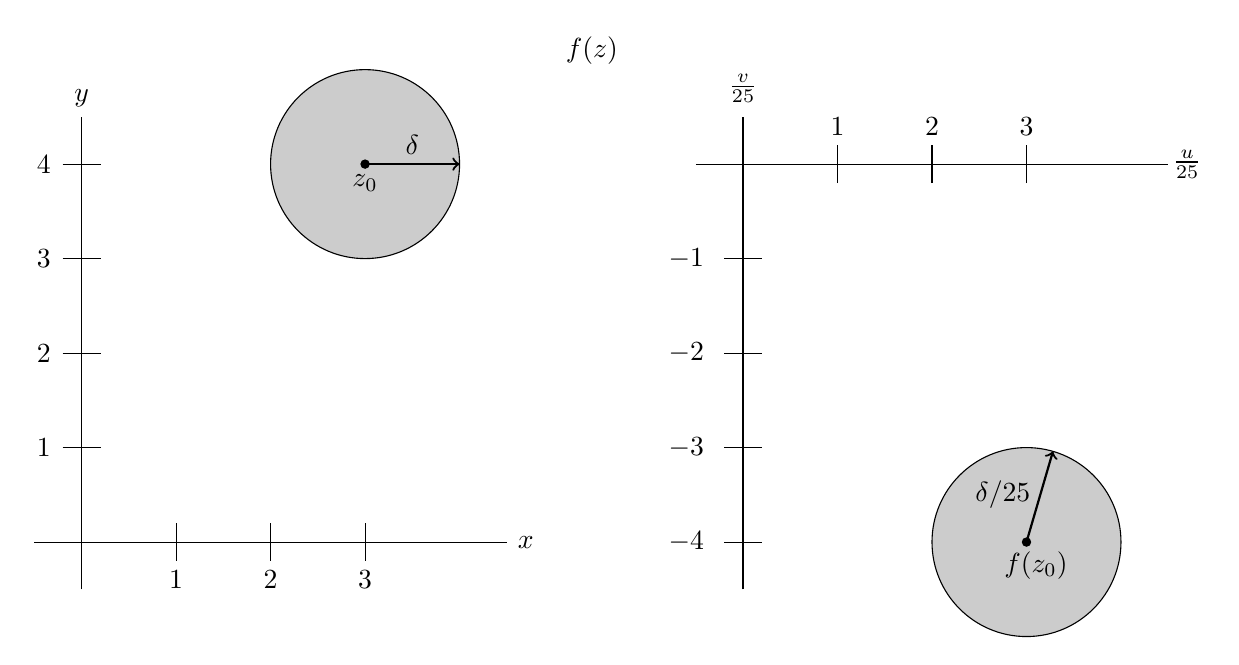
\begin{tikzpicture} [scale=1.2]
      %XY-PLANE
      \draw[-] (-5,0) -- (0,0); %draw axes 1
      \draw[-] (-4.5,-0.5) -- (-4.5,4.5);
      \draw[-] (-4.7,1) -- (-4.3,1); %y-axis ticks
      \draw[-] (-4.7,2) -- (-4.3,2);
      \draw[-] (-4.7,3) -- (-4.3,3);
      \draw[-] (-4.7,4) -- (-4.3,4);
      \draw[-] (-3.5,-0.2) -- (-3.5,0.2); %x-axis ticks
      \draw[-] (-2.5,-0.2) -- (-2.5,0.2);
      \draw[-] (-1.5,-0.2) -- (-1.5,0.2);
      \node at (-4.9,1) {$1$}; %y-axis numbers
      \node at (-4.9,2) {$2$};
      \node at (-4.9,3) {$3$};
      \node at (-4.9,4) {$4$};
      \node at (-3.5,-0.4) {$1$}; %x-axis numbers
      \node at (-2.5,-0.4) {$2$};
      \node at (-1.5,-0.4) {$3$};

      \draw[->,thick] (3-4.5,4) -- (4-4.5,4); %draw delta vec
      \draw (3-4.5,4) circle(1cm); %draw circle edge
      \fill[opacity=0.2] (3-4.5,4) circle[radius=1cm]; %draw circle fill

      \fill (3-4.5,4) circle[radius=0.05cm]; %draw labels
      \node at (3-4.5,3.8) {$z_0$};
      \node at (3.5-4.5,4.2) {$\delta$};
      \node at (0.2,0) {$x$};
      \node at (-4.5,4.7) {$y$};

      \centerarc[thick,<-](0.9,4)(45:135:1); %draw mapping arrow
      \node at (0.9,5.2) {$f(z)$};

      %UV-PLANE
      \draw[-] (2,4) -- (7,4); %draw axes 2
      \draw[-] (2.5,-0.5) -- (2.5,4.5);
      \draw[-] (-4.7+7,1) -- (-4.3+7,1); %y-axis ticks
      \draw[-] (-4.7+7,2) -- (-4.3+7,2);
      \draw[-] (-4.7+7,3) -- (-4.3+7,3);
      \draw[-] (-4.7+7,0) -- (-4.3+7,0);
      \draw[-] (-3.5+7,-0.2+4) -- (-3.5+7,0.2+4); %x-axis ticks
      \draw[-] (-2.5+7,-0.2+4) -- (-2.5+7,0.2+4);
      \draw[-] (-1.5+7,-0.2+4) -- (-1.5+7,0.2+4);
      \node at (-4.9+6.8,0) {$-4$}; %y-axis numbers
      \node at (-4.9+6.8,1) {$-3$};
      \node at (-4.9+6.8,2) {$-2$};
      \node at (-4.9+6.8,3) {$-1$};
      \node at (-3.5+7,0.4+4) {$1$}; %x-axis numbers
      \node at (-2.5+7,0.4+4) {$2$};
      \node at (-1.5+7,0.4+4) {$3$};

      \draw[->,thick] (3+2.5,0) -- (3+2.5+0.28,0.96); %draw delta vec
      \draw (3+2.5,0) circle(1cm); %draw circle edge
      \fill[opacity=0.2] (3+2.5,0) circle[radius=1cm]; %draw circle fill

      \fill (3+2.5,0) circle[radius=0.05cm]; %draw labels
      \node at (3+2.6,-0.25) {$f(z_0)$};
      \node at (3.5+1.75,0.5) {$\delta/25$};
      \node at (0.2+7,4) {$\frac{u}{25}$};
      \node at (-4.5+7,4.8) {$\frac{v}{25}$};
    \end{tikzpicture}
    \end{center}
\end{mdframed}


\item (10) Describe the projection on the Riemann Sphere of the set $\{z = x + iy : x \geq \sqrt{3}\}$. I encourage you to include a nice diagram.

\begin{mdframed}
  If $Z = (x_1,\,x_2,\,x_3)$ is the projection on the Riemann sphere of the point $z = x + iy$ in the complex plane, then
  \begin{equation*}
    x_1 = \frac{2\,\text{Re}\,z}{|z|^2 + 1},
    \qquad x_2 = \frac{2\,\text{Im}\,z}{|z|^2 + 1},
    \qquad x_3 = \frac{|z|^2 - 1}{|z|^2 + 1}.
  \end{equation*}
  Let us first start by determining what the line $(x,y) = (\sqrt{3},y)$ projects to on the Riemann sphere. Since all lines and cirlces in the $z$-plane correspond under stereographic projection to cirlces on the Riemann sphere, we are really just trying to figure out {\it which} circle the line projects to. The point $Z$ has coordinates
  \begin{equation*}
    x_1 = \frac{2\sqrt{3}}{4 + y^2},
    \qquad x_2 = \frac{2y}{4 + y^2},
    \qquad x_3 = \frac{2 + y^2}{4 + y^2}.
  \end{equation*}
  When $y=0$, we find that $Z = (\sqrt{3}/2,0,1/2)$. In the limit that $y\rightarrow\pm\infty$, the projected points approach the north pole $Z\rightarrow(0,0,1)$ from the $\pm$ $y$-direction. The norm of the separation vector $(\sqrt{3}/2,0,1/2) - (0,0,1) = (\sqrt{3}/2,0,-1/2)$ is 1, meaning that the circle projected on the surface has radius 0.5 (note that here we aren't considering the distance {\it on} the sphere, but in the $3$-space the sphere is embedded in). We could also set the $y$-derivative of the $x_2$ equation to zero to find the minimum and maximum values of $x_2$ (which turn out to be $x_2 = \pm 0.5$). So, for $x = \sqrt{3}$, we get a circle of radius 0.5 centered at $Z = (1/2,0,\sqrt{3}/2)$. A slice of the sphere corresponding to $x_2 = 0$ is shown below. The dark arc on the circle from $\theta = \pi/6$ to $\theta = \pi/2$, as measured from the positive $x_1$-axis, displays the portion of the sphere the circle is on.

  \begin{center}
  \begin{tikzpicture} [scale=3]
  \draw[-] (-1.4,0) -- (2,0); %draw axes
  \draw[-] (0,-1.4) -- (0,1.4);
  \draw[-,opacity=0.5] (0,0) -- (0.866,0.5);
  \draw[opacity=0.3] (0,0) circle(1cm); % draw circle
  \centerarc[ultra thick,-](0,0)(30:90:1);
  \centerarc[thick,->,opacity=0.5](0,0)(0:30:0.8);
  \draw[dotted,-,thick] (0,1) -- (0.866,0.5);
  \draw[dotted,-,very thick] (2*0.866,0) -- (0.866,0.5);

  %draw labels
  \node at (2.15,0) {$x_1$};
  \node at (0,1.55) {$x_3$};
  \node at (1.025,0.2) {$\theta = \pi/6$};

  \draw[-] (0.866*2,-0.1) -- (0.866*2,0.1);
  \node at (0.866*2,-0.2) {$\sqrt{3}$};
 \end{tikzpicture}
  \end{center}

  If we were to continue doing this for every value of $x$ greater than $\sqrt{3}$, we would find that every subsequent line maps to a circle inside the circle mapped out by the line $x = \sqrt{3}$. Thus, the set $\{z = x + iy : x \geq \sqrt{3}\}$ projects to the circle of radius 0.5 centered at $Z = (1/2,0,\sqrt{3}/2)$ and all points on the sphere within that circle. A visualization of this projection is shown below, wherein the blue circle and the black line bordering it are the projections of the given set. The line $x = \sqrt{3}$ is shown in the bottom right, along with three points and their projections (connected by the dotted lines).

  \begin{center}
  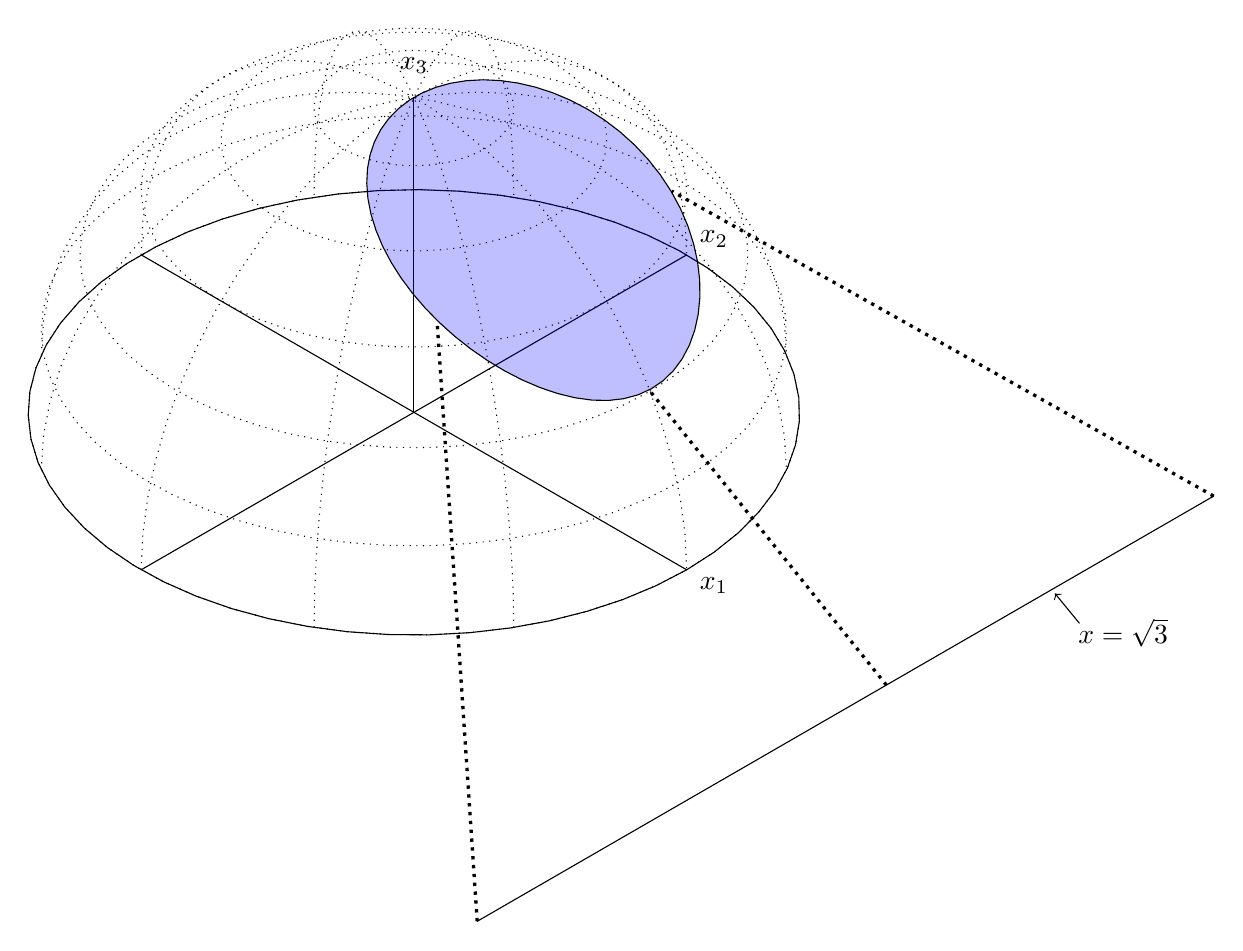
\begin{tikzpicture}[x=(-30:4cm),y=(30:4cm),z=(90:4cm)]

  \def\R{1}

  \draw (1.732,-1.5,0) -- (1.732,1.2,0); %x=sqrt{3}
    \draw[->] (1.89,0.55,0) -- (1.75,0.6,0);
    \node at (2,0.6,0) {$x = \sqrt{3}$};
  \draw[dotted,-,very thick] (1.732,-1.5,0) -- (0.5,-0.415,0.745);
  \draw[dotted,-,very thick] (1.732,1.2,0) -- (0.51,0.435,0.74);
  \draw[dotted,-,very thick] (1.732,0,0) -- (0.866,0,\R/2);

  \draw (-\R,0,0) -- (\R,0,0);
    \node at (1.1*\R,0,0) {$x_1$};
  \draw (0,-\R,0) -- (0,\R,0);
    \node at (0,1.1*\R,0) {$x_2$};
  \draw (0,0,0) -- (0,0,\R);
    \node at (0,0,1.1*\R) {$x_3$};
  \draw plot [domain=0:360, samples=60, variable=\i] 
      (\R*cos \i, \R*sin \i, 0) -- cycle;

  \def\r{0.432}

  \foreach \i in {0, 30,...,150}
      \draw [dotted] plot [domain=-90:90, samples=30, variable=\j]        
          (\R*cos \i*sin \j,\R*sin \i*sin \j, \R*cos \j);

  \foreach \j in {0, 15,...,90}
      \draw [dotted] plot [domain=0:360, samples=60, variable=\i]  
              (\R*cos \i*sin \j,\R*sin \i*sin \j, \R*cos \j);

  \foreach \cr in {0.432}
      \foreach \ca [evaluate={\cx=\cr*cos \ca; \cy=\cr*sin \ca;}]in {0.8}
          \draw [black, fill=blue, fill opacity=.25] 
              plot [domain=0:360, samples=60, variable=\t] 
                  (\cx+\r*cos \t,\cy+\r*sin \t, {sqrt(\R^2-(\cx+\r*cos(\t))^2-(\cy+\r*sin(\t))^2)})
                      -- cycle;

  \end{tikzpicture}
  \end{center}
\end{mdframed}


\item (15) Choose one of the following explorations.
\begin{enumerate}
  \addtocounter{enumii}{1}
  \item  An exploration of {\it admissibility}. Recall that if $z = x + iy$, then $x = \frac{1}{2}(z + \bar{z})$ and $y = \frac{1}{2i}(z - \bar{z})$.
  
  \begin{enumerate}
  \item (4) Substitute for $x$ and $y$ in $f(x,y) = x^2 - y^2 + i2xy$ and verify that $f$ reduces to a function of $z$ only, i.e. that there are no $\bar{z}$ terms remaining after simplification. Also use the Cauchy Riemann Equations to verify that $f$ is analytic.

  \begin{mdframed}
  Using the relationships $x = \frac{1}{2}(z + \bar{z})$ and $y = \frac{1}{2i}(z - \bar{z})$, we obtain
  \begin{align*}
    f(x,y) &= \left(\frac{z + \bar{z}}{2}\right)^2 - \left(\frac{z - \bar{z}}{2i}\right)^2 + i2\left(\frac{z + \bar{z}}{2}\right)\left(\frac{z + \bar{z}}{2i}\right) \\
    &= \frac{1}{4}(z^2 + \bar{z}^2 + 2 z \bar{z}) + \frac{1}{4}(z^2 + \bar{z}^2 - 2 z \bar{z}) + \frac{1}{2}(z^2 - \bar{z}^2) \\
    &= \frac{1}{4}(z^2 + \bar{z}^2 + 2 z \bar{z} + z^2 + \bar{z}^2 - 2 z \bar{z} + 2z^2 - 2\bar{z}^2) \\
    &= \frac{1}{4}(4z^2) \\
    &= z^2.
  \end{align*}
  Now, we turn our attention to the Cauchy-Riemann equations
  \begin{equation*}
    \frac{\partial u}{\partial x} = \frac{\partial v}{\partial y} \qquad\text{and}\qquad \frac{\partial u}{\partial y} = -\frac{\partial v}{\partial x},
  \end{equation*}
  where $u$ and $v$ denote the real and imaginary parts, respectively, of $f(x,y)$. For our function:
  \begin{align*}
    \frac{\partial u}{\partial x} = 2x, \quad&\qquad \frac{\partial v}{\partial y} = 2x, \\
    \frac{\partial u}{\partial y} = -2y, \;&\qquad \frac{\partial v}{\partial x} = 2y.
  \end{align*}
  Since the first partial derivatives are continuous and satisfy the Cauchy-Riemann equations at all points of $\mathbb{C}$, $f$ is entire.
  \end{mdframed}

    
  \item (4) Substitute for $x$ and $y$ in $g(x,y) = x^2 - y^2 + i 3 x y$ and verify that $f$ does not reduce to a function of $\bar{z}$ only, i.e. that there are still $\bar{z}$ terms remaining after simplification. Also use the Cauchy Riemann Equations to verify that $g$ is not analytic.

  \begin{mdframed}
  Using the relationships $x = \frac{1}{2}(z + \bar{z})$ and $y = \frac{1}{2i}(z - \bar{z})$, we obtain
  \begin{align*}
    g(x,y) &= \left(\frac{z + \bar{z}}{2}\right)^2 - \left(\frac{z - \bar{z}}{2i}\right)^2 + i3\left(\frac{z + \bar{z}}{2}\right)\left(\frac{z + \bar{z}}{2i}\right) \\
    &= \frac{1}{4}(z^2 + \bar{z}^2 + 2 z \bar{z}) + \frac{1}{4}(z^2 + \bar{z}^2 - 2 z \bar{z}) + \frac{3}{4}(z^2 - \bar{z}^2) \\
    &= \frac{1}{4}(z^2 + \bar{z}^2 + 2 z \bar{z} + z^2 + \bar{z}^2 - 2 z \bar{z} + 3z^2 - 3\bar{z}^2) \\
    &= \frac{1}{4}(5z^2 - \bar{z}^2) \\
    &= \frac{5}{4}z^2 - \frac{1}{4}\bar{z}^2.
  \end{align*}
  Evaluating the Cauchy-Riemann equations for this function yields
  \begin{align*}
    \frac{\partial u}{\partial x} = 2x, \quad&\qquad \frac{\partial v}{\partial y} = 3x, \\
    \frac{\partial u}{\partial y} = -2y, \;&\qquad \frac{\partial v}{\partial x} = 3y.
  \end{align*}
  Since the Cauchy-Riemann equations are satsified nowhere, the function $g(x,y)$ is nowhere analytic.
  \end{mdframed}

  \item (7) {\it Admissibility} essentially boils down to the idea that $f(x,y) = u(x, y) + iv(x, y)$ does not depend on $z$. A more precise way to say this is that $\frac{\partial f}{\partial \bar{z}} = 0$. Use the multivariable chain rule,
  \begin{equation*}
    \frac{\partial f}{\partial \bar{z}} = \frac{\partial f}{\partial x} \frac{\partial x}{\partial \bar{z}} + \frac{\partial f}{\partial y} \frac{\partial y}{\partial \bar{z}},
  \end{equation*}
  to show that $\frac{\partial f}{\partial \bar{z}} = 0$ if the Cauchy Riemann Equations are satisfied. This indicates that $f$ does not depend on $\bar{z}$ if $f$ is analytic.

  \begin{mdframed}
  First, note that $\partial x/\partial \bar{z} = 1/2$ and $\partial y/\partial \bar{z} = i/2$. Next, substitute $f = u + iv$ into the given equation:
  \begin{align*}
    \frac{\partial f}{\partial \bar{z}} &= \frac{\partial f}{\partial x} \frac{\partial x}{\partial \bar{z}} + \frac{\partial f}{\partial y} \frac{\partial y}{\partial \bar{z}} \\
    &= \frac{1}{2}\frac{\partial(u + iv)}{\partial x} + \frac{i}{2}\frac{\partial (u + iv)}{\partial y} \\
    &= \frac{1}{2}\left(\frac{\partial u}{\partial x} +i\frac{\partial v}{\partial x}\right) + \frac{i}{2}\left(\frac{\partial u}{\partial y} +i\frac{\partial v}{\partial y}\right) \\
    &= \frac{1}{2}\left[\left(\frac{\partial u}{\partial x} - \frac{\partial v}{\partial y}\right) + i\left(\frac{\partial u}{\partial y} + \frac{\partial v}{\partial x}\right)\right].
  \end{align*}
  Regarding the last line, the expressions in parentheses are zero, and thus $\frac{\partial f}{\partial \bar{z}} = 0$, when the Cauchy-Riemann equations are satisfied. We conclude that if a function is analytic, then it has no $\bar{z}$-dependence.
  \end{mdframed}

  \end{enumerate}
\end{enumerate}

\end{enumerate}

\end{document}